\documentclass[10pt]{article}

\usepackage[letterpaper,margin=0.82in]{geometry}
\usepackage[T1]{fontenc}
\usepackage[utf8]{inputenc}
\usepackage{lmodern}
\usepackage{microtype}
\usepackage{amsmath,amssymb,mathtools}
\usepackage{booktabs,tabularx,array,longtable}
\usepackage{enumitem}
\usepackage[round,authoryear]{natbib}
\usepackage{xcolor}
\usepackage{url}
\usepackage{hyperref}
\usepackage{tikz}
\usetikzlibrary{arrows.meta,positioning,fit,shapes.geometric}

% Evidence values are kept in one file so the manuscript cannot silently drift
% from the final verification record. Update this file only from reproduced runs.
\newcommand{\shadisplay}[8]{\texttt{sha256:#1}\allowbreak\texttt{#2}\allowbreak\texttt{#3}\allowbreak\texttt{#4}\allowbreak\texttt{#5}\allowbreak\texttt{#6}\allowbreak\texttt{#7}\allowbreak\texttt{#8}}
\newcommand{\ArtifactVersion}{1.0.0}
\newcommand{\EvidenceDate}{2026-08-09}
\newcommand{\CoreSuiteSummary}{Ruff check and 125-file format check, strict mypy on 32 source files, uv lock check, and container build-context policy passed}
\newcommand{\CoreTestsCollected}{409}
\newcommand{\CoreTestSummary}{407 passed; 2 e2e deselected; 75.41\% branch-aware coverage}
\newcommand{\CompatibilitySummary}{Python 3.11.15: 407 passed, 2 deselected, 75.39\% branch-aware coverage}
\newcommand{\PackageSummary}{two byte-identical wheel/sdist builds, Twine and isolated import/CLI checks passed; Bandit 1.9.4 \code{-ll} and pip-audit 2.10.1 clean}
\newcommand{\WheelBytes}{206,347}
\newcommand{\WheelDigest}{sha256:30d68c41b311526870d534c863696c2bcefc7b639b3784e54f3ce5cded63566c}
\newcommand{\WheelDigestDisplay}{\shadisplay{30d68c41}{b3115268}{70d534c8}{63696c2b}{cefc7b63}{9b3784e5}{4f3ce5cd}{ed63566c}}
\newcommand{\SdistBytes}{189,923}
\newcommand{\SdistDigest}{sha256:3f66fb8642956fe750d52e27c36458045f3d3d44ee44c00ddd8b79d566535b85}
\newcommand{\SdistDigestDisplay}{\shadisplay{3f66fb86}{42956fe7}{50d52e27}{c3645804}{5f3d3d44}{ee44c00d}{dd8b79d5}{66535b85}}
\newcommand{\CoverageFloor}{74\%}
\newcommand{\ProductionAcceptanceResult}{passed}
\newcommand{\ProductionAcceptanceDuration}{41.894 seconds}
\newcommand{\ProductionRuntimeImageDigest}{sha256:336feda3da169ecffea8ab3f0b68858c5de304cafe2208ee696d714c6dab64c4}
\newcommand{\ProductionRuntimeImageDigestDisplay}{\shadisplay{336feda3}{da169ecf}{fea8ab3f}{0b68858c}{5de304ca}{fe2208ee}{696d714c}{6dab64c4}}
\newcommand{\ProductionRuntimeImageID}{sha256:5d397bb16c6da91199595f2344fcabc109f08af69ca02b5d5bc4c3bf8245eb38}
\newcommand{\ProductionRuntimeImageIDDisplay}{\shadisplay{5d397bb1}{6c6da911}{99595f23}{44fcabc1}{09f08af6}{9ca02b5d}{5bc4c3bf}{8245eb38}}
\newcommand{\ProductionEvidenceBytes}{4,414}
\newcommand{\ProductionEvidenceDigest}{sha256:e9d8c47ab92b26c78c20552038be38641ba509047183ea7f36b1c34d0dbd353b}
\newcommand{\ProductionEvidenceDigestDisplay}{\shadisplay{e9d8c47a}{b92b26c7}{8c205520}{38be3864}{1ba50904}{7183ea7f}{36b1c34d}{0dbd353b}}
\newcommand{\ProductionManifestDigest}{sha256:80ebcdba5ae7d27f94248564b59c68dd75aaecceda70572eb301ec632acb40de}
\newcommand{\ProductionManifestDigestDisplay}{\shadisplay{80ebcdba}{5ae7d27f}{94248564}{b59c68dd}{75aaecce}{da70572e}{b301ec63}{2acb40de}}
\newcommand{\ProductionSourceDigest}{sha256:ba0ede68f6def3244bebe9a051239fc34a28f76f0cfb324d0816cc50714cf06f}
\newcommand{\ProductionSourceDigestDisplay}{\shadisplay{ba0ede68}{f6def324}{4bebe9a0}{51239fc3}{4a28f76f}{0cfb324d}{0816cc50}{714cf06f}}
\newcommand{\ProductionSourceCount}{167}
\newcommand{\ProductionSourceCommit}{\texttt{8cd4b5e2f50c5d356de249aa93af2aef516e1fa6}}
\newcommand{\ProductionSQLiteVersion}{3.53.2}
\newcommand{\ProductionTransferred}{10}
\newcommand{\ProductionAuditRecordCounts}{6, 5, and 1}
\newcommand{\ProductionSignerInvocations}{21, 9, and 4}
\newcommand{\ModelCheckBounds}{scalar budget 3; three wardens; at most three leases, two transfers, and two receipts; unit actions; depth 9}
\newcommand{\ModelCheckSummary}{101,245 states, 318,558 transitions, and 66,072 idempotent self-loops; zero invariant violations}
\newcommand{\ModelCheckTableSummary}{passed; 101,245 states}
\newcommand{\TLCCheckSummary}{40,057 generated states, 6,776 distinct states, maximum depth 14, and an empty queue}
\newcommand{\TLCCheckTableSummary}{passed; 6,776 distinct states}
\newcommand{\MutationCheckSummary}{a three-action prepare, accept, duplicate-accept counterexample at depth 2}
\newcommand{\StorageBenchmarkSummary}{100 operations/path; FULL durability}
\newcommand{\BenchmarkEnvironment}{Windows 10 build 19045; Python 3.14.0; SQLite 3.50.4; AMD64; 32 logical CPUs}
\newcommand{\BenchmarkSourceCommit}{\texttt{9f6ba18315c1a1ba854373053f7bd92e18343e9b}}
\newcommand{\BenchmarkAuthorize}{8.2877 & 9.3887 & 119.24}
\newcommand{\BenchmarkPrepare}{7.48085 & 8.6475 & 130.57}
\newcommand{\BenchmarkAccept}{6.9838 & 7.8025 & 137.74}
\newcommand{\BenchmarkFinalize}{6.484 & 7.615 & 151.56}
\newcommand{\BenchmarkRoundTrip}{21.08745 & 23.1221 & 46.48}
\newcommand{\BenchmarkVerify}{0.17805 & 0.1829 & 5,577.09}
\newcommand{\BenchmarkClaim}{4.41765 & 5.8287 & 219.34}
\newcommand{\BenchmarkContention}{56.4619 & 69.5167 & 49.02}
\newcommand{\BenchmarkContentionPninetyfive}{69.5167}
\newcommand{\ScalingAuthorizeMedians}{6.96635, 7.17425, 8.48515, and 10.52645 ms}
\newcommand{\InvariantAggregateMedians}{1.3121, 1.29235, and 1.2494 ms}
\newcommand{\KeeperRatio}{1.139237}
\newcommand{\KeeperPenalty}{13.92\%}
\newcommand{\LockedPackages}{48}
\newcommand{\LockBytes}{315,852}


\definecolor{letsblue}{HTML}{185FA5}
\definecolor{letsteal}{HTML}{0F766E}
\definecolor{letsorange}{HTML}{B45309}
\definecolor{letsgrey}{HTML}{4B5563}
\definecolor{letslight}{HTML}{EFF6FF}
\hypersetup{
  colorlinks=true,
  linkcolor=letsblue,
  citecolor=letsteal,
  urlcolor=letsblue,
  pdftitle={LETS: A Distributed Runtime for Lineage-Bounded Autonomous Systems},
  pdfauthor={AstralDeep LETS Contributors}
}
\urlstyle{same}
\setlist{nosep,leftmargin=1.5em}
\setlength{\parindent}{1.1em}
\setlength{\parskip}{0.12em}
\setlength{\tabcolsep}{5pt}
\renewcommand{\arraystretch}{1.13}
\emergencystretch=2em

\newcommand{\LETS}{\textsc{LETS}}
\newcommand{\impl}{\textsc{Implemented}}
\newcommand{\measured}{\textsc{Measured}}
\newcommand{\checked}{\textsc{Checked}}
\newcommand{\designed}{\textsc{Designed}}
\newcommand{\future}{\textsc{Future}}
\newcommand{\vect}[1]{\boldsymbol{#1}}
\newcommand{\code}[1]{\nolinkurl{#1}}
\newcommand{\status}[1]{\textcolor{letsblue}{\textsf{#1}}}

\title{\vspace{-1.5em}\textbf{LETS: A Distributed Runtime for\\Lineage-Bounded Autonomous Systems}\\[0.55em]
\large System paper and artifact report for version \ArtifactVersion}
\author{AstralDeep LETS Contributors\\
\small Standalone Apache-2.0 implementation at \url{https://github.com/AstralDeep/LETS}}
\date{\EvidenceDate}

\begin{document}
\maketitle

\begin{abstract}
Autonomous systems increasingly create descendants, delegates, replicas, services, and robots
that act concurrently and may remain useful while disconnected. Qualitative authorization alone
does not bound the aggregate quantity of effects that a recursively changing population can
produce, while a central counter makes disconnected work unavailable. We present Lineage Escrow
Transition Systems (\LETS), a standalone distributed authorization runtime. A fixed set of stable
warden processes owns disjoint shares of a finite, multi-dimensional envelope. Ephemeral subjects
receive signed, expiring leases whose resources and capabilities can only be attenuated. Protected
effects are state-machine transitions; a warden atomically debits a transition and emits a
short-lived, audience-bound receipt that an independent executor verifies and durably claims.

This paper reports the implemented version \ArtifactVersion{} runtime rather than the earlier
in-memory research kernel. It includes independent SQLite-backed warden processes, signed cluster
manifests, authenticated peer HTTP, sequenced exactly-once target credit for rights transfers,
branch revocation, canonical signed JSON, externally anchored warden and executor authority,
bounded maintenance, an authenticated HTTP API and a strict-decoding, bounded-retry client,
authority-safe immutable observation snapshots, quiescence-first terminal restart fencing,
pre-cleanup failure-evidence harvesting, operational tooling, and a host-neutral adapter. We give an inductive
conservation argument and state the availability cost:
a partitioned site may spend only rights it already owns, so safety and local progress are
preserved while remote capacity can be stranded. The artifact contains \CoreTestsCollected{}
collected unit, integration, security, property, recovery, and end-to-end cases. A final one-host
production-profile acceptance used the exact immutable candidate with three hardened wardens; it
exercised mTLS and JWT rejection paths, a bidirectional partition, abrupt restart, automatic
convergence, an externally anchored executor replay store, stale-restore rejection, and aggregate
conservation. The repository also supplies a separately hardened,
one-warden-per-host production profile whose admission depends on operator-provided storage,
identity, key, PKI, and rollback-domain controls. This is not a claim of Byzantine tolerance,
arbitrary live migration, generic exactly-once physical effects, or independent security audit.
\end{abstract}

\noindent\fcolorbox{letsblue}{letslight}{\parbox{0.95\linewidth}{
\textbf{Claim discipline.} \impl{} denotes behavior present in the source artifact;
\measured{} denotes a reproduced observation with a recorded environment; \checked{} denotes
tests, property exploration, or a bounded abstract state-space check; \designed{} denotes a
protocol argument that is not a mechanized proof; and \future{} denotes work outside version
\ArtifactVersion. These labels prevent architecture, tests, and measurements from being reported
as interchangeable forms of evidence.
}}

\section{Introduction}

Agent replication is an authority-allocation problem before it is a copying problem. A child may
be created by cloning code, starting a process, delegating a task, launching a container, or
instantiating a robot controller. None of those mechanisms determines how much authority the
resulting population can exercise. A parent that gives each child its full quota amplifies
authority; a shared eventually consistent counter can overspend during a partition; and a central
authorization service sacrifices disconnected progress.

\LETS{} treats spawn as one governed transition in a more general lineage lifecycle. Its core
object combines: (i) a finite integer resource vector; (ii) qualitative capabilities; (iii) an
immutable transition machine; (iv) nested expiries and branch revocation; and (v) distributed
escrow held by stable wardens. The system is reasoner-independent. An LLM, symbolic planner,
workflow engine, or fixed controller can propose the same transition. Safety depends on complete
mediation at a warden and protected executor, not on model compliance.

The component ideas are established. Database escrow partitions rights so local transactions can
preserve numeric invariants \citep{oneil1986escrow}; bounded counters extend this idea to
eventually consistent systems \citep{balegas2015bounded}; exactly-once quantity transfer addresses
duplicate delivery \citep{shoker2015exactlyonce}; and finite quota can be recursively delegated
\citep{agudo2009quota}. Capabilities, attenuated credentials, state machines, and runtime security
automata are likewise prior art \citep{saltzer1975protection,birgisson2014macaroons,andersen2019wave,harel1987statecharts,schneider2000enforceable}.
The contribution is a narrow composition and its operational realization: stable escrow replicas
are separated from churn-heavy lineage subjects, protected effects are receipts for funded state
transitions, and rights move between wardens through a durable protocol rather than by copying an
active subtree.

\subsection{Contributions and non-claims}

This artifact makes six concrete contributions.

\begin{enumerate}
  \item \impl{} A real multi-node runtime in which each warden has an independent process,
  database, signing identity, monotonic authority anchor, audit archive, and initial escrow share
  in the production profile. Schema~2 makes peer replay part of the same anchored core authority.
  \item \impl{} A durable lifecycle and transition service that provides root issuance, recursive
  attenuating spawn, renewal, quiescence, closure, expiry reclamation, branch revocation, and
  signed executor receipts under atomic local transactions.
  \item \impl{} A signed, sequenced rights-transfer protocol with idempotent target acceptance,
  bounded reordering, acknowledgements, and bilateral prefix checkpoints.
  \item \designed{} An inductive safety argument for local and global vector conservation,
  capability attenuation, nested expiry, and receipt mediation, together with an explicit
  partition-availability trade-off.
  \item \impl{} A bounded observation and restart-evidence lane that publishes one coherent,
  authority-bound snapshot without request-path database admission, quiesces workload requests
  before terminal fencing, and permits process replacement only after an exact durable fence proof.
  \item \checked{} Reproducible unit, security, property, crash-recovery, bounded-model, package,
  and real three-node fault evidence, with the evidence types kept distinct.
\end{enumerate}

\LETS{} does not claim that escrow, delegation, state machines, signatures, leases, or
hash-chained audit are individually novel. It does not claim Byzantine safety, automatic policy
correctness, instant offline revocation, transparent active-subtree migration, or exactly-once
physical effects from a receipt alone.

\subsection{From research kernel to distributed runtime}

The original manuscript described an in-memory Python kernel and a proposed deployment. Version
\ArtifactVersion{} replaces that implementation claim with a persisted service and preserves the
old kernel only as historical material. Table~\ref{tab:status} summarizes the boundary.

\begin{table}[ht]
\centering
\caption{Evidence status in version \ArtifactVersion.}
\label{tab:status}
\small
\begin{tabularx}{\linewidth}{@{}p{0.18\linewidth}X p{0.18\linewidth}@{}}
\toprule
Area & Artifact status & Evidence class \\
\midrule
Local lifecycle & Durable lease, policy, receipt, audit, idempotency, and outbox transactions & \impl, \checked \\
Multi-node transfer & Signed prepare/accept/finalize/checkpoint protocol over authenticated HTTP & \impl, \checked \\
Partition behavior & Both directed A--B peer links disabled with a durable failed transfer record; dispatcher converged after restoration & \measured \\
Restart behavior & Warden process replaced on its persisted authority unit; anchored state resumed and transfer converged & \measured \\
Conservation & Inductive argument, SQL commit checks, property traces, bounded abstract checker, aggregate e2e assertion & \designed, \checked \\
Rollback fencing & Database-instance and append-only history heads compared through external linearizable anchors & \impl, \checked \\
Observation and restart & Immutable authority-bound snapshots, freshness failure, quiescence-first fence proof, and bounded pre-cleanup evidence & \impl, \checked \\
Production profile & Admission requires one warden per host, mTLS, external providers, independent state/anchor/audit/backup domains, and an immutable image digest; one-host acceptance emulates the controls but not independent failure domains & \impl, \checked{} (one host) \\
Byzantine wardens & No threshold authorization or replicated-state-machine defense & \future \\
Active-subtree migration & Free-right transfer followed by target issuance only & \future \\
\bottomrule
\end{tabularx}
\end{table}

\section{System Model and Requirements}

\subsection{Entities and trust boundaries}

Let $W$ be a configured, bounded set of wardens. Each warden is a stable accounting process with
its own durable database and Ed25519 signing identity. Let $L$ be the dynamic set of leases issued
to agents or other subjects. Membership in $L$ can grow and shrink recursively; membership in $W$
changes only through an operator-controlled configuration epoch.

An envelope is named by $(tenant, envelope, epoch)$ and fixes an ordered resource schema. For
$m$ dimensions, resource values are elements of
$\mathcal{R}_m = \{0,\ldots,2^{63}-1\}^m$ with componentwise order and checked arithmetic. A
policy binds that schema to one immutable state machine, lease and receipt time bounds, a clock
uncertainty bound, an evidence predicate language, and a transfer gap window. Policies and
machines are content addressed.

The trusted computing base consists of each warden process, its policy and configured evidence
evaluators, database, clock within the configured uncertainty, signing provider, manifest trust
roots, production authority-anchor and audit-archive services, protected executors and their
claim anchors, the TLS/identity termination boundary, and the host isolation that prevents
subjects from writing those components.
Agents, generated code, prompts, memory, discovery documents, request bodies, networks, and other
tenants are untrusted. Wardens are trusted but may crash. Messages may be lost, duplicated,
delayed, reordered, replayed, or partitioned.

\begin{figure}[ht]
\centering
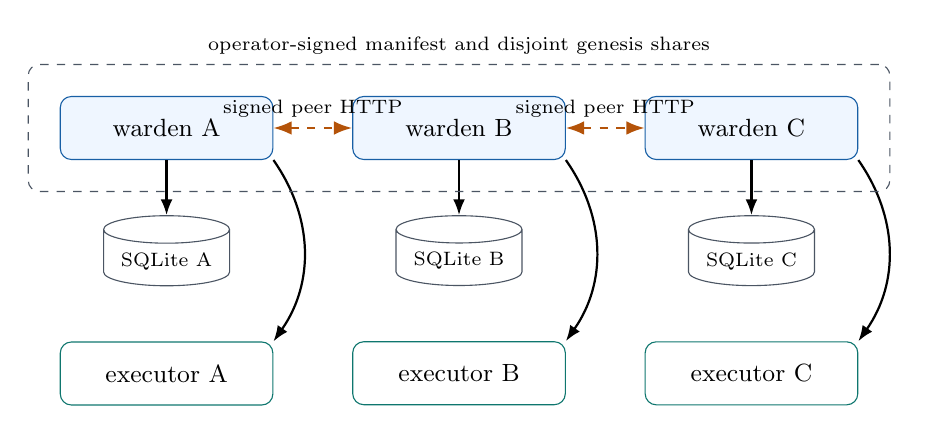
\begin{tikzpicture}[
  node distance=7mm and 10mm,
  box/.style={draw=letsblue,rounded corners,fill=letslight,minimum width=27mm,minimum height=8mm,align=center,font=\small},
  db/.style={draw=letsgrey,cylinder,shape border rotate=90,aspect=0.25,minimum width=16mm,minimum height=8mm,align=center,font=\scriptsize},
  exec/.style={draw=letsteal,rounded corners,minimum width=27mm,minimum height=8mm,align=center,font=\small},
  arr/.style={-{Latex[length=2mm]},thick},
  peer/.style={<->,>=Latex,thick,dashed,draw=letsorange}
]
\node[box] (a) {warden A};
\node[box,right=of a] (b) {warden B};
\node[box,right=of b] (c) {warden C};
\node[db,below=of a] (da) {SQLite A};
\node[db,below=of b] (db) {SQLite B};
\node[db,below=of c] (dc) {SQLite C};
\node[exec,below=of da] (ea) {executor A};
\node[exec,below=of db] (eb) {executor B};
\node[exec,below=of dc] (ec) {executor C};
\draw[peer] (a) -- node[above,font=\scriptsize]{signed peer HTTP} (b);
\draw[peer] (b) -- node[above,font=\scriptsize]{signed peer HTTP} (c);
\draw[arr] (a) -- (da); \draw[arr] (b) -- (db); \draw[arr] (c) -- (dc);
\draw[arr] (a.south east) to[out=-55,in=55] (ea.north east);
\draw[arr] (b.south east) to[out=-55,in=55] (eb.north east);
\draw[arr] (c.south east) to[out=-55,in=55] (ec.north east);
\node[draw=letsgrey,dashed,rounded corners,fit=(a)(b)(c),inner sep=4mm,label={[font=\scriptsize]above:operator-signed manifest and disjoint genesis shares}] {};
\end{tikzpicture}
\caption{Reference topology. The acceptance deployments instantiate three independent warden
processes, stores, and keys. The production profile additionally separates each warden database,
monotonic authority anchor, audit archive, and backup domain; its protected executor similarly
separates schema-5 replay state from the executor anchor. Ephemeral subjects call wardens but are
not escrow replicas.}
\label{fig:topology}
\end{figure}

\subsection{Safety and availability requirements}

The principal safety property is that no execution schedule creates resource rights. Spawn and
transfer may relocate rights; a transition may move them into consumed accounting; reclamation
may return unconsumed rights; no operation may increase the global envelope. Capability and
machine authority must attenuate down a lineage, lease expiry must be nested, and an executor must
reject an invalid, stale, wrongly addressed, or replayed receipt.

Availability is conditional. A healthy warden should authorize from its local share without a
peer round trip. Under a partition, a site can continue only while it has locally escrowed rights,
valid leases, a sufficiently certain clock, and a reachable protected executor. Remote rights are
not borrowed speculatively. This chooses bounded authority over full utilization during every
partition.

\section{LETS Design}

\subsection{Local ownership equation}

For warden $w$, let $\vect{S}_w$ be its signed genesis share, $\vect{I}_w$ cumulative accepted
inbound transfer, $\vect{F}_w$ its free pool, $\vect{R}_w$ the sum of residual rights in
unreclaimed leases, $\vect{C}_w$ cumulative consumption, and $\vect{O}_w$ cumulative prepared
outbound transfer. The persisted local invariant is
\begin{equation}
  \vect{S}_w + \vect{I}_w
  = \vect{F}_w + \vect{R}_w + \vect{C}_w + \vect{O}_w.
  \label{eq:local}
\end{equation}
Every term is a nonnegative vector of the same dimension. The manifest verifies
$\sum_w \vect{S}_w = \vect{B}$, where $\vect{B}$ is the global initial budget. Since an inbound
credit can exist only for a signed, already prepared source voucher, define the source-owned
in-flight vector on a consistent cut as
$\vect{X}=\sum_w(\vect{O}_w-\vect{I}_w)$. Summing Eq.~\ref{eq:local} yields
\begin{equation}
  \vect{B}
  = \sum_w (\vect{F}_w + \vect{R}_w + \vect{C}_w) + \vect{X}.
  \label{eq:global}
\end{equation}
Before target acceptance, transferred rights are in $\vect{X}$; after acceptance, matching
outbound and inbound cumulative terms cancel. This formulation avoids counting a prepared
voucher as both source capacity and target capacity.

\subsection{Signed leases and recursive attenuation}

A lease grant binds tenant, envelope, epoch, lease and lineage identifiers, parent and subject,
original allocation, capabilities, policy and machine digests (the latter committing to the
initial machine state), ancestor path, branch epoch, issue and expiry times, warden and key
identifiers, and a signature. The
mutable snapshot contains residual vector, current state, lifecycle status, and monotonically
increasing sequence.

Root issuance is a privileged operation: a transport-authenticated identity must hold
\code{lets.admin}, \code{lets.warden.admin}, or \code{lets.lease.issue}. It debits the local free
pool and cannot request a capability absent from the bound machine; the allocation must contain at
least one positive component. Spawn is available to the authenticated parent subject or an identity holding
\code{lets.admin} or \code{lets.lease.manage}. A child allocation is likewise nonzero. For parent
$p$ and child $c$, the transaction requires
\begin{align}
  \vect{a}_c &\leq \vect{r}_p, &
  K_c &\subseteq K_p, \\
  t^{exp}_c &\leq t^{exp}_p, &
  d^{policy}_c &= d^{policy}_p,\quad d^{machine}_c=d^{machine}_p.
\end{align}
It then atomically replaces $\vect{r}_p$ by $\vect{r}_p-\vect{a}_c$ and creates the child with
residual $\vect{a}_c$. A request cannot substitute a cheaper or more permissive machine behind a
different policy identifier. Expected state and sequence fields provide optimistic concurrency
guards. A durable request identifier is unique envelope-wide across mutation types; its full
fingerprint makes retries idempotent and rejects a same-key/different-operation or body collision.

Replication has deliberately narrow semantics. It creates a new governed runtime identity and
partitions authority. It does not copy bearer tokens, private keys, human identity, process memory,
open sockets, uncommitted state, protected data, or signing secrets. Artifact and workspace
transfer remain host operations.

\subsection{Transition authorization and protected execution}

Each protected transition specifies source state, target state, required capability, a
componentwise nonnegative resource cost with at least one positive component, and an optional
declarative evidence rule. The evidence language is data, not executable policy code; policy and
machine digests include its semantics. Evidence can satisfy a guard but cannot mint resources or
capabilities.

After the network boundary authenticates the request and the service validates the identity object,
authorization performs the following stateful checks and mutations in one local write transaction:
\begin{enumerate}
  \item tenant/subject/scope binding; lease status, branch epoch, expiry, and clock checks;
  \item request-id fingerprint lookup and optional expected state/sequence checks;
  \item immutable policy/machine resolution, legal transition, capability, audience, and evidence
  evaluation;
  \item componentwise residual debit and machine state/sequence update;
  \item signed receipt, idempotent response, hash-chained audit event, and outbox persistence; and
  \item durable commit before returning the receipt.
\end{enumerate}

The protected executor has a separate trust configuration and replay database. It always verifies
the exact audience, receipt freshness under bounded clock uncertainty, and signature against a
registered warden/key pair that is currently valid at verification time. Local
\code{ExecutorPolicy} fields and allowlists can further pin tenant, envelope, epoch, policy
digest, machine digest, and warden.

The production-grade SQLite executor library profile uses schema~5. One immutable replay identity
binds the exact audience, tenant, envelope, configuration epoch, hash of the complete executor
policy, and hash of the complete verification-key registry. Each successful claim appends a
digest-chained history record and advances a database-instance-bound claim head and clock floor. A
linearizable external compare-and-swap anchor must acknowledge that committed head before the
claim returns; an older restore, divergent copy, losing concurrent clone, policy widening, or
verification-key substitution therefore fails closed. Live receipt and lease-watermark rows are
each pruned in batches of at most 128 (up to 256 rows across the two tables per successful claim),
but the authority claim chain is append-only and requires capacity planning for a finite executor
epoch. Schema~4 has no promotable external claim history; transition to schema~5 requires a
drained, newly initialized authority unit. The repository's production Compose unit runs wardens,
not an executor service; applications must host the executor, its independent state and anchor,
and its atomic or idempotent physical-effect integration.

The claim requires the lease sequence to advance and claims both receipt identifier and nonce.
This supplies at-most-once authorization consumption. A generic receipt cannot make an arbitrary
physical effect exactly once: the executor must bind receipt claim and effect in one domain
transaction, make the effect idempotent, or use compensation.

\subsection{Lifecycle and revocation}

Quiescence disables transition execution without inventing a second policy-machine state. Resume
restores actionability if the lease remains valid. Renewal is bounded by the policy maximum and by
the parent expiry; a root renewal additionally requires \code{lets.lease.manage} or
\code{lets.admin}. Version \ArtifactVersion{} refuses parent shortening that would strand a live longer-lived
descendant. Close and expiry reclamation return only the lease's own residual, once.
Reclamation waits past clock uncertainty and the maximum outstanding receipt lifetime so a receipt
cannot remain valid after its authority has been reassigned.

A branch revocation is a signed monotonic epoch for a lineage/branch prefix. Only the branch-owning
warden may create it; authenticated peers may relay the owner-signed record. Connected descendants
fail closed once the revocation is visible. A disconnected descendant cannot be revoked instantly
without communication. Its additional resource exposure is nevertheless bounded componentwise by
the residual already present in that branch, and its time exposure is bounded by nested lease
expiry plus the configured clock/receipt safety margin under complete mediation. This is an
engineering bound, not a claim that a compromised executor or bypass path is contained.

\section{Cross-Warden Rights Transfer}

\subsection{Protocol}

For each $(source,target,envelope)$ stream, the source allocates strictly increasing sequence
numbers. The protocol is a durable handoff, not a distributed transaction spanning both databases.

\begin{figure}[ht]
\centering
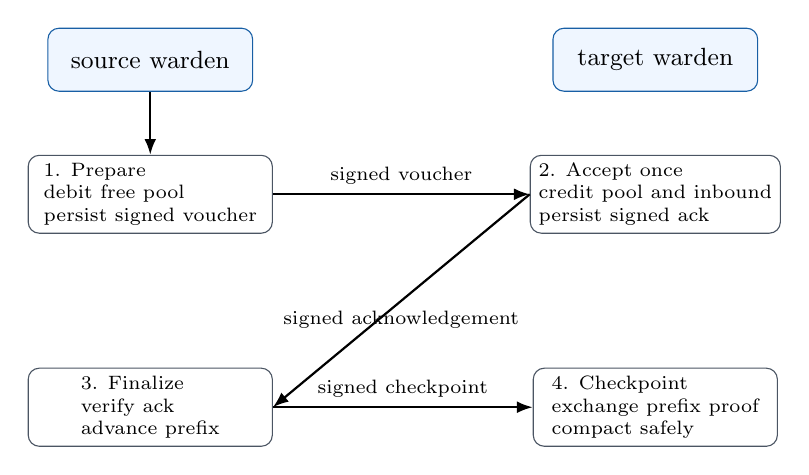
\begin{tikzpicture}[
  actor/.style={draw=letsblue,rounded corners,fill=letslight,minimum width=26mm,minimum height=8mm,align=center,font=\small},
  note/.style={draw=letsgrey,rounded corners,minimum width=31mm,align=left,font=\scriptsize,inner sep=3pt},
  arr/.style={-{Latex[length=2mm]},thick},
  node distance=8mm and 17mm
]
\node[actor] (s) {source warden};
\node[actor,right=38mm of s] (t) {target warden};
\node[note,below=of s] (p) {1. Prepare\\debit free pool\\persist signed voucher};
\node[note,below=of t] (a) {2. Accept once\\credit pool and inbound\\persist signed ack};
\node[note,below=17mm of p] (f) {3. Finalize\\verify ack\\advance prefix};
\node[note,below=17mm of a] (c) {4. Checkpoint\\exchange prefix proof\\compact safely};
\draw[arr] (s) -- (p);
\draw[arr] (p.east) -- node[above,font=\scriptsize]{signed voucher} (a.west);
\draw[arr] (a.west) -- node[below,font=\scriptsize]{signed acknowledgement} (f.east);
\draw[arr] (f.east) -- node[above,font=\scriptsize]{signed checkpoint} (c.west);
\end{tikzpicture}\par
\caption{Transfer ownership moves monotonically. A timeout never refunds a prepared source
voucher; retries recover the acknowledgement without a second target credit.}
\label{fig:transfer}
\end{figure}

\paragraph{Prepare.} The source atomically subtracts the amount from its free pool, increments
cumulative outbound accounting, assigns the next sequence, and persists a signed voucher. A
timeout does not restore the amount. Before target acceptance it remains source-owned in-flight
authority in Eq.~\ref{eq:global}, but it is no longer spendable.

\paragraph{Accept.} The target authenticates both the peer HTTP message and the signed voucher,
checks tenant/envelope/epoch/source/target/policy binding, and enforces a bounded gap window.
Unique sequence and transfer-id bindings prevent alternate payloads. The first valid acceptance
credits the free pool and cumulative inbound accounting in one transaction and stores a signed
acknowledgement. A business-level duplicate returns the stored logical acknowledgement without a
second credit; an exact replay of the signed HTTP envelope is rejected by the durable nonce store.

\paragraph{Finalize and checkpoint.} The source verifies the target signature and voucher digest,
records finalization idempotently, and advances a contiguous acknowledgement watermark. Once both
peers agree on a finalized contiguous prefix, a signed checkpoint permits deletion of individual
rows below that prefix. Gaps, conflicting identifiers, backward watermarks, unknown epochs, and
untrusted keys fail closed.

Watermark advance and physical history deletion are deliberately incremental: each contiguous-
prefix or physical-prune maintenance primitive processes at most 64 transfer-history rows per
invocation; direct record and conflict checks are separate. An exact duplicate acknowledgement,
voucher, or checkpoint can drive the next bounded watermark or maintenance batch without a second
credit or new signature. Branch-revocation materialization and expiry reclamation are likewise
limited to 64 leases per transaction; dispatcher and audit-export work use configured bounded
batches (64 by default). These limits bound individual WAL/write sets while repeated work
converges.

For audit export, each record reaches the idempotent archive before local acknowledgement. The
sink-committed prefix is then acknowledged in one reserved authority-serialized transaction per
batch, rather than one authority admission per record. A crash before the batch commit leaves the
published prefix pending for exact repair from the archive head; no record is acknowledged before
its archive write succeeds. Each export cycle also carries a two-second publish budget measured
from cycle start: an expiring budget acknowledges the prefix published so far, and follow-up
cycles run immediately whenever a cycle was truncated or its snapshot filled the batch, skipping
the archive-head call and prefix acknowledgement because the head is exactly the record just
acknowledged; every fresh cycle refetches the head, preserving rollback detection. The budget
can only take effect between publishes; the archive-head call, one in-flight publish, and the
busy-bounded acknowledgement transactions each retain their own five-second allowances, so the
fault-free depth-one worst case for a record that just misses a batch snapshot is 36 seconds,
and the declared 40-second export staleness bound dominates it while deeper backlogs drain at
publish throughput.

\impl{} A running warden's bounded peer dispatcher discovers authoritative transfer, revocation,
and checkpoint records through durable delivery metadata. It schedules one head per ordered
stream, signs HTTP requests, retries failed delivery with bounded exponential delay, finalizes
acknowledged transfers, creates checkpoints, and prunes only terminal delivery metadata. Work is
not lost if the process crashes between the authority transaction and dispatcher discovery.
At-least-once peer delivery remains conditional on connectivity, a live trusted peer, and both
signing keys remaining current; idempotent receiving converts redelivery into exactly-once
accounting credit, not exactly-once network transmission.

\subsection{Failure outcomes}

Table~\ref{tab:failures} states the intended result, including the availability cost.

\begin{table}[ht]
\centering
\caption{Transfer and partition outcomes. ``Safe'' means no duplicated spendable rights under the
trusted-warden model; it does not imply liveness.}
\label{tab:failures}
\small
\begin{tabularx}{\linewidth}{@{}p{0.26\linewidth}X p{0.14\linewidth}@{}}
\toprule
Failure & Result & Property \\
\midrule
Voucher lost after prepare & Amount stays unspendable at source; retry same durable voucher & Safe, unavailable \\
\addlinespace
Acknowledgement lost & Redelivery returns stored acknowledgement; target is not credited twice & Safe, retryable \\
\addlinespace
Out-of-order delivery within window & Target records gap; contiguous watermark advances when missing prefix arrives & Safe, bounded memory \\
\addlinespace
Gap beyond window or conflicting sequence & Request rejected & Fail closed \\
\addlinespace
Target crash after commit & Persisted credit, acknowledgement, and replay state recover on reopen & Safe after recovery \\
\addlinespace
Peer partition & Each warden continues only from local rights; transfer stalls & Safe, partial progress \\
\addlinespace
Signer reaches finite \code{not_after} with pending records & Verification continues to fail closed; prepared rights or revocation/checkpoint delivery can remain stranded & Safe, unavailable \\
\addlinespace
Concurrent source database/key clones & Production anchor admits one contiguous history branch and faults the loser; unanchored development can duplicate authority & Fail closed \\
\bottomrule
\end{tabularx}
\end{table}

\section{Implementation}

The implementation is a typed Python package supporting Python 3.11--3.14 \citep{lets2026}. The
core depends on \code{PyNaCl}~1.6.2 over libsodium for Ed25519; optional server and client extras
provide FastAPI/Uvicorn and HTTPX. Development dependencies are resolved by the committed lockfile
into a repository-local \code{.venv}. Containers build an image-local environment and do not mount
the host environment.

\subsection{Durable storage and atomicity}

Each SQLite database owns one envelope. It uses foreign keys, write-ahead logging,
\code{synchronous=FULL}, a bounded busy timeout, schema/application identifiers, migrations,
startup integrity checks, and \texttt{BEGIN IMMEDIATE} for serialized writes \citep{sqlitewal}.
Checked vector functions are registered with SQLite. Triggers maintain the lease-residual
aggregate and validate dimensions; a transaction-level pre-commit check rejects a local
conservation violation. Compound foreign keys prevent mixing a policy version with another digest.
The authoritative tables cover metadata, warden state, immutable policies, leases, receipts,
idempotency responses, revocations, inbound and outbound transfer streams, checkpoints, signed
audit, and outbox state. Core schema~2 also owns peer-HTTP nonce claims, their monotonic clock
floor, revision, and history digest. An exact schema-1 migration refuses to proceed while any
legacy claim remains live. Once all have expired, it binds the legacy artifact digest and clock
floor into the new history, advances the new floor to at least the migration time, and never opens
the retired file as live state again. The runtime does not make those retired bytes immutable;
operators must protect the exact verified backup and migration journal as evidence.

Production opens require an external linearizable authority anchor outside the database rollback
domain. A checkpoint binds warden/envelope/epoch, schema, signing-key fingerprint, random database
instance, audit head, state revision/digest, and clock floor. Storage reconciles before every
transaction and after each committed write; an acknowledged write result is not released ahead of
the post-commit compare-and-swap.
The database can recover a committed local extension, but an older or divergent restore and a
losing clone cannot pass admission against the advanced anchor.

The capacity contract distinguishes logical from physical limits. \code{max_database_bytes}
installs SQLite \code{max_page_count} on every connection and caps the logical main database; it
does not cap the live WAL or shared-memory index. Before an authority write, LETS reserves the
emergency filesystem floor plus all remaining main-file growth, a conservative transaction that
could write every configured page to WAL, and additional WAL-index growth. It also retains a
logical page reserve inside the main-file ceiling. Capacity recovery paths remain available only
within this reserve. \code{SQLITE_FULL}, including when raised by checkpointing, becomes a sticky
fail-closed fault; other checkpoint failures are surfaced explicitly. Operators must provide an
exclusive quota or dedicated filesystem for the free-space reading to be meaningful. The contract
is conservative headroom, not a throughput or retention guarantee.

The storage abstraction admits another backend, but only SQLite has equivalent implementation and
fault evidence in this release. The release dependency audit selected PyNaCl/libsodium for the
signed path and removed an unused PostgreSQL extra; version \ArtifactVersion{} exposes neither a
PostgreSQL dependency nor a validated adapter.

The supplied deployment validator and production server admission reject a SQLite runtime that
lacks the 2026 WAL-reset safety fix and explicitly reject the withdrawn 3.52 release line. Older
SQLite measurements in Section~\ref{sec:evaluation} are development-only algorithmic observations,
not evidence that such a runtime is production-admissible.

\subsection{Canonical signed data and key trust}

All content digests and signatures use the documented \code{LETS-CJ/1} profile. Object keys are
sorted by Unicode scalar value, arrays retain order, integer values are lossless signed 64-bit
values, and output is minimal UTF-8 JSON. Floats, non-finite values, duplicate keys, non-string
keys, lone surrogates, and non-canonical base64url spellings are rejected. \code{LETS-CJ/1} is
intentionally not RFC~8785 JCS because nanosecond timestamps and resource values may exceed the
lossless integer range of common IEEE-754 JSON consumers \citep{rfc8785}. Cross-language
implementations must use the published conformance vectors and lossless parsing.

Signed-record type tags use the LETS-owned \code{lets.*} version namespace; the cluster manifest
uses \code{lets.manifest/v1}. Neither the core protocol nor its canonical bytes contain an
AstralDeep-specific type namespace.

Ed25519 authority records bind both warden and key identifiers. The trust registry rejects
conflicting registrations. Manifest-bound service startup, readiness, and every authority-record
signing path require the complete declared clock-uncertainty interval to fit within the signer's
configured not-before/not-after interval; peer receivers independently enforce current-time key
validity for protocol records and signed HTTP requests. A new policy registration applies the
authority-signing rule before commit. The cluster manifest
binds the envelope schema, global budget, exact disjoint shares, peer endpoints, keys, and policies;
local bootstrap trust configuration fixes the accepted operator keys and required signature
threshold. Manifest verification counts distinct operator key material rather than aliases, requires
warden key identifiers and Ed25519 public-key material to be globally unique, and forbids Ed25519
public-key material reuse across operator and online warden roles. Non-loopback plain HTTP endpoints
require an explicit development override;
production deployment requires TLS in addition to message signatures.

The warden database never stores the private signing seed. Its immutable bootstrap metadata binds
the initial warden/key identifier and SHA-256 public-key fingerprint; signing-key identity or
public-key material substitution therefore fails startup. Manifest-backed service startup reloads
strict JSON and re-verifies the manifest
digest, operator threshold, local key/configuration, and complete peer trust before serving.

Version 1 resource limits bound adversarial parser and validation work: at most 256 resource
dimensions, 1,024 machine transitions, 64 ancestor-path entries, and evidence expression depth 32
with at most 256 nodes and 256 membership values per node. These are protocol limits, not measured
capacity guidance.

\subsection{Network planes}

The client plane strictly decodes JSON and rejects unknown top-level fields in endpoint request
bodies; deliberately opaque evidence and configuration values remain open, and dynamic policy
registration performs targeted semantic checks but does not enforce the complete nested OpenAPI
\code{Policy} schema. The published OpenAPI~3.1 artifact documents closed request schemas for clients,
endpoint 2xx response schemas, and \code{application/problem+json} errors. Runtime handlers produce
those responses, but the bundled client does not validate success bodies against OpenAPI. Identity
is derived by an injected authenticator, never accepted from body fields. The
bundled static bearer authenticator is development bootstrap tooling and stores only token digests.

Production selects exactly one installed \code{lets.runtime_providers} entry point. The provider
must return the exact tenant/warden, a signer, authenticator, independent authority anchor,
independently durable audit sink, and an exact \code{production_capable} declaration. The built-in
raw-seed/static-bearer provider is forbidden. The bundled vendor-neutral provider calls an
operator-controlled Ed25519 signer helper without a shell, verifies short-lived EdDSA JWTs, and
uses separately mounted file anchor and SQLite audit archive. Those local bindings make the
profile runnable; a cloud KMS, PKCS\#11 device, OIDC/SPIFFE identity plane, remote linearizable
anchor, and managed archive remain operator-installed integrations, not bundled conformance.

Authentication is enforced at the network boundary. Direct calls to service and administrative
ports are trusted in-process integration calls, not authenticated remote entry points; an embedding
host must keep them inside its TCB.

Peer requests carry method, raw target path/query, body digest, timestamp, nonce, warden, key, and
an Ed25519 signature. Schema~2 claims each nonce in an externally anchored core write before
handler execution, prunes at most 128 expired claims per request, and advances a digest-bound
replay clock floor. That nonce write is not atomic with the later peer business operation, so a
valid request can consume its nonce even if the handler subsequently rejects or fails. Peer
signatures authenticate content but do not provide confidentiality or hide
metadata. Production serving requires inbound mTLS and HTTPS manifest endpoints; peer-enabled
nodes additionally require hostname-verifying outbound TLS with a client certificate. Certificate
issuance, revocation policy, and identity lifecycle are deployment responsibilities. TLS and the
bundled generic provider's JWT trust are loaded at process startup, so their certificate, key, and
trust rotation requires controlled process recreation with a configured overlap interval; the
Python TLS path does not perform online OCSP validation. In the bundled profile, mTLS channel
admission and JWT or LETS signed-message
authorization are independent checks: the JWT is not bound to the presented client certificate,
and tenant/scopes are not derived from its subject or SAN. Certificate-bound workload identity
requires an operator provider or gateway integration. The generic authenticator requires a
syntactically valid \code{jti} but does not persist or consume it; the same bearer JWT can therefore
be replayed until its expiry plus accepted skew. Revocation and one-time-token semantics likewise
require an operator identity or gateway integration.

The operator surface provides liveness, bounded clock-aware readiness, invariant snapshots, audit
verification, bounded audit pagination, and metrics for pools, consumption, transfer
watermarks/gaps, capacity, and outbox lag. A background exporter reconciles the core audit chain
with an independently durable, identity-bound contiguous archive. The exporter waits at most a
configured deadline for each sink call; a timed-out call may continue in its single daemon worker,
and later publication attempts fail while that worker remains live. Blocked publication,
divergence, excess backlog, or stalled progress makes production readiness false. Export
acknowledgement and outbox pruning are bounded and resumable. The signed core audit chain itself is
immutable and retained; export is rollback/recovery evidence, not permission to delete history.

Production backup creates an exclusively published recovery bundle only after a durable drain and
empty peer/audit queues. The bundle contains configuration, the core database, any required legacy
replay artifact, the signed manifest, and checkpoint metadata. It intentionally excludes the live
authority anchor, audit archive, signer/provider recovery material, identity keys, and PKI; those
external dependencies require their own coordinated recovery procedures. Restore begins from a
separately trusted live configuration and signed manifest and requires the bundled copies to be
byte-identical; it does not adopt lost configuration or perform an epoch migration. It validates a
scratch copy, compares it non-mutatingly with the current anchor before publication, moves the old
core/WAL/SHM sidecars into quarantine across resumable phases, and removes that quarantine after
successful admission. The restored node remains drained until explicit operator activation. These
mechanisms fence stale state; they do not make simultaneous copies an endorsed topology. The
bundled recovery path covers warden core authority only, not schema-5 executor replay state or its
claim anchor. Executor recovery is application-operated: fence effects, snapshot the replay
database, retain the anchor separately, and require an anchored reopen.

\subsection{Authority-safe observation and terminal replacement}

Production health cannot safely bypass authority ordering by reading the SQLite WAL directly: a
database commit can become visible before the external anchor compare-and-swap has acknowledged
the branch. Version~\ArtifactVersion{} instead constructs an immutable observation through one
priority, authority-safe read admission. The capture binds the database identity, authority
lifetime and checkpoint, core revision, audit head and verifier state, runtime readiness,
conservation vectors, peer/exporter state, schema hashes, and monotonic capture time into a
canonical snapshot digest. Request handling serves that process-local snapshot asynchronously,
without another storage admission or shared worker-thread hop. A capture failure immediately makes
the retained document unready; age beyond the 15-second bound is returned explicitly as stale
rather than hidden behind a transport timeout.

Planned replacement separates preparation from the 30-second process-replacement window. The
workload first quiesces at a completed request boundary. The host then validates an exact terminal
audit proof and re-inspects the unchanged container before a durable container-clock
acknowledgement binds the terminal proof and target identity. Only after that acknowledgement may
the host issue \code{SIGKILL}; replacement identity, authority lifetime, checkpoint lineage, and
completion are then checked within the acknowledged bound. The one-hour release harness retains
bounded health, workload, coordination, resource, and failure diagnostics before it removes the
scenario volume. These records support offline validation; they do not make the host clock and
container monotonic clock numerically interchangeable.

\subsection{Module decomposition}

\begin{table}[ht]
\centering
\caption{Major implementation boundaries.}
\label{tab:modules}
\small
\begin{tabularx}{\linewidth}{@{}p{0.25\linewidth}X@{}}
\toprule
Module & Responsibility \\
\midrule
\code{policy}, \code{models} & Immutable transition/evidence semantics and strict signed wire records \\
\code{service} & Lifecycle, transition, revocation, transfer, invariant, and audit transactions \\
\code{storage.sqlite} & Versioned schema, durability/capacity admission, repositories, conservation checks, and core replay authority \\
\code{crypto}, \code{canonical} & Ed25519 trust and \code{LETS-CJ/1} bytes/digests \\
\code{auth}, \code{api}, \code{client}, \code{peer} & Transport identity, signed HTTP/replay defense, durable peer dispatch, and client/CLI contracts \\
\code{executor}, \code{executor_authority} & Independent receipt verification, schema-5 at-most-once claim, and external rollback anchor \\
\code{authority}, \code{audit}, \code{recovery} & Warden monotonic CAS, independent contiguous audit export, and journaled bundles/restore \\
\code{observation} & Priority coherent capture, incremental audit verification, immutable freshness-bound publication, and terminal audit proof \\
\code{runtime}, \code{providers} & Selected signer/identity/anchor/audit provider contract and bundled generic profile \\
\code{manifest} & Operator-signed cluster bootstrap and exact genesis-share validation \\
\code{integrations} & Host-neutral lifecycle port and optional AstralDeep scope profile \\
\bottomrule
\end{tabularx}
\end{table}

\section{Safety Argument}

This section is a protocol-level inductive argument, not a machine-checked refinement proof. The
bounded checker and executable tests discussed in Section~\ref{sec:evaluation} provide separate,
finite evidence.

\subsection{Local conservation}

\textbf{Lemma 1 (local preservation).} If Eq.~\ref{eq:local} holds before a committed operation,
each implemented operation preserves it componentwise.

\textit{Argument.} Root issuance moves a vector from $\vect{F}_w$ to $\vect{R}_w$. Spawn moves a
vector between parent and child terms inside $\vect{R}_w$. An authorized transition moves its cost
from $\vect{R}_w$ to $\vect{C}_w$. Close or reclamation moves a residual from $\vect{R}_w$ to
$\vect{F}_w$. Quiescence, resume, renewal, and revocation change status or time metadata but not
resource terms. Prepare subtracts from $\vect{F}_w$ and adds to $\vect{O}_w$. Target acceptance
adds the same voucher amount to both $\vect{F}_w$ and $\vect{I}_w$. Finalization and checkpointing
change no vector. Retried idempotent operations return the prior result; rejected or rolled-back
operations change no authoritative state. Checked arithmetic prevents wraparound. \hfill$\square$

\textbf{Theorem 1 (global conservation under the failure model).} If the signed manifest exactly
partitions $\vect{B}$, all wardens begin in a locally valid state, peer keys are trusted, and every
committed operation is one of the operations above, then Eq.~\ref{eq:global} holds on every
consistent cut despite crash, retry, duplication, reordering, loss, or partition.

\textit{Argument.} Lemma~1 preserves every local equality. A target increments $\vect{I}$ only
after verifying a matching signed prepared voucher; uniqueness constraints prevent a second
credit. Therefore cumulative inbound never creates an unmatched source debit. Summation and the
manifest share equation yield Eq.~\ref{eq:global}. Message failures affect whether a prepared term
moves out of $\vect{X}$, not whether it is duplicated. \hfill$\square$

The theorem excludes a compromised warden signing nonexistent vouchers, manifest trust-root
compromise, and direct database modification. Production admission adds a linearizable external
anchor: two database/key clones may race, but only one contiguous history branch can advance and
the loser faults before returning an acknowledged authorization. This fencing argument depends on
anchor availability, independence from the database snapshot, and correct compare-and-swap
semantics; it is not Byzantine replication.

\subsection{Lineage and transition properties}

\textbf{Lemma 2 (attenuation).} Along every issued lineage edge $p\rightarrow c$, the child's
capability set is a subset of the parent's, the immutable policy/machine digests are equal, the
child expiry is no later than the parent's, and the child allocation is removed from the parent in
the same transaction.

\textit{Argument.} These are explicit preconditions and writes of the spawn transaction. Subject
binding prevents an unscoped sibling from invoking spawn on another lease. The policy digest and
machine digest are signed into the grant. \hfill$\square$

\textbf{Lemma 3 (transition soundness).} Under complete mediation and uncompromised trusted code,
an executor accepts a receipt only for a committed transition whose source state, capability,
evidence, vector cost, policy/machine digests, audience, sequence, and validity interval passed the
warden checks.

\textit{Argument.} The debit, state/sequence update, signed receipt, idempotency response, and audit
record commit atomically. The executor independently verifies all signed bindings and atomically
claims the receipt. In production its external claim anchor must acknowledge the append-only head
before the claim is returned. A missing, invalid, stale, divergent, or replayed receipt/claim state
fails closed. \hfill$\square$

Lemma~3 says nothing about the semantic adequacy of a configured cost or evidence predicate, nor
about effects reachable through a bypassable executor.

\section{Evaluation and Reproducible Evidence}
\label{sec:evaluation}

The evaluation asks whether the implementation satisfies its protocol obligations under bounded
and adversarial schedules. It is not a claim of external security certification or broad workload
performance.

\subsection{Evidence layers}

\begin{table}[ht]
\centering
\caption{Verification layers and what they can establish.}
\label{tab:evidence}
\small
\begin{tabularx}{\linewidth}{@{}p{0.22\linewidth}p{0.24\linewidth}X@{}}
\toprule
Layer & Reproduced status & Scope and limitation \\
\midrule
Static checks & \CoreSuiteSummary & Ruff formatting/lint and strict mypy check source consistency; neither proves protocol safety. \\
Test suite & \CoreTestSummary & Unit, integration, security, property, concurrency, crash, and recovery behavior; finite executions only. \\
Compatibility/package & \CompatibilitySummary; \PackageSummary & One additional interpreter and isolated artifact/import checks; not a platform certification. \\
TLA+ TLC & \TLCCheckTableSummary & Scalar three-warden escrow/transfer/receipt kernel; finite and not a source-code refinement. \\
Bounded checker & \ModelCheckTableSummary & \ModelCheckBounds; abstracts signatures, clocks, SQL, and HSM labels. \\
Production acceptance & \ProductionAcceptanceResult{} in \ProductionAcceptanceDuration & Exact-digest candidate under one-host Linux Compose; mTLS, hardening, partition, restart, convergence, and anchored executor checks, not independent failure domains. \\
Sustained production profile & \SoakResult{} for \SoakMeasurementDuration; \SoakHealthSamples{} health samples & One seeded exact-candidate run with bounded partitions and replacements; not a capacity benchmark or independent-failure-domain trial. \\
Microbenchmarks & \StorageBenchmarkSummary & Development measurements only; no cross-system baseline unless reported with environment and repetitions. \\
\bottomrule
\end{tabularx}
\end{table}

\subsection{Bounded formal exploration}

The artifact supplies a finite TLA+ specification of scalar escrow, transfer, receipt, and replay
semantics \citep{lamport1994tla}. TLC completed its configured TypeOK and conservation checks with
\TLCCheckSummary. A separate dependency-free executable abstract model explores root issuance,
recursive spawn, consumption, close/reclamation, sequenced transfer preparation, reordering,
acceptance, finalization, receipt claim, and duplicate delivery. Under \ModelCheckBounds, it
explored \ModelCheckSummary. A fault-injection mode that credits an already accepted transfer found
\MutationCheckSummary. The latter is a checker-sensitivity test, not evidence that the production
implementation contains that fault. Both models abstract signatures, clocks, SQL, HTTP, and key
labels; neither is an unbounded proof or a refinement check against the runtime. Executable service
trace conformance is tested, not proved as a refinement mapping.

Property tests independently generate checked-vector inputs and randomized lifecycle traces.
Security cases target privilege boundaries, policy substitution, request-id collision, evidence
type confusion, concurrent parent overdraw, transfer identity/sequence conflicts, signature
spelling, peer key validity, executor races, and canonical wire parsing. Recovery cases open a
database after rollback, committed transaction, and abrupt process exit.

The release candidate's serial non-e2e gate ran with \code{ResourceWarning} promoted to an error:
\CoreTestSummary. The
two Docker e2e cases are reported separately so an unavailable Docker daemon cannot be hidden
inside the core-suite result. Required compatibility CI produced \CompatibilitySummary. Two clean,
archive-derived package builds produced byte-identical artifacts; Twine, wheel-content and RECORD
validation, exact source/archive parity, isolated base/server/client wheel and sdist imports, CLI
startup on Python~3.14, Bandit~1.9.4 at medium/high severity, and pip-audit~2.10.1 passed. These are
bounded tool results, not an external security certification. Hosted CI for acceptance source
commit \ProductionSourceCommit{} completed green. The wheel was
\WheelBytes{} bytes with digest \WheelDigestDisplay; the source distribution was \SdistBytes{} bytes
with digest \SdistDigestDisplay; and the exact 16-file deployment bundle was \DeploymentBytes{}
bytes with digest \DeploymentDigestDisplay.

\subsection{Frozen 1.0.0 storage measurements}

\measured{} The reviewed baseline used \BenchmarkEnvironment{} and the release PyNaCl/libsodium
backend. Each main path ran 10 warm-up and 100 measured operations with \code{perf_counter_ns} and
nearest-rank percentiles. Every writing path kept SQLite WAL \code{synchronous=FULL} and one atomic
transaction per stage; verify-only has no write. The clean committed benchmark worktree recorded
\code{git_worktree_dirty=false} at \BenchmarkSourceCommit; its metadata cross-references the clean
acceptance source-tree digest. That commit differs from the accepted source commit only in retained
evidence files. The single-host in-process measurements exclude HTTP, network, container
scheduling, external authority/audit services, and independent failure domains. Its
SQLite~3.50.4 runtime is not production-admissible under the release gate. The reviewed
machine-readable baseline is retained under \code{benchmarks/baselines}.

\begin{table}[ht]
\centering
\caption{Frozen 1.0.0 development-path latency and wall-time rate. The 100-sample p95 values are indicative,
not capacity guarantees.}
\label{tab:benchmarks}
\small
\begin{tabularx}{\linewidth}{@{}Xrrr@{}}
\toprule
Path & Median (ms) & p95 (ms) & Rate (op/s) \\
\midrule
Warden authorize & \BenchmarkAuthorize \\
Transfer prepare & \BenchmarkPrepare \\
Transfer accept & \BenchmarkAccept \\
Transfer finalize & \BenchmarkFinalize \\
Transfer round trip & \BenchmarkRoundTrip \\
Executor verify only & \BenchmarkVerify \\
Executor verify and durable claim & \BenchmarkClaim \\
Four-worker authorize contention & \BenchmarkContention \\
\bottomrule
\end{tabularx}
\end{table}

Authorization includes validation, evidence/policy evaluation, Ed25519 signing, audit, invariant
maintenance, and durable commit. The transfer round trip is three FULL transactions across two
stores and excludes HTTP/network time. The four-worker row uses independent leases in one
single-writer database; latency includes lock wait, and its \BenchmarkContentionPninetyfive-ms p95 shows why
the result must not be generalized to arbitrary write concurrency.

\impl{} The final optimization pass removed an unconditional full
\texttt{PRAGMA foreign\_key\_check} from every successful write while retaining per-connection foreign
key enforcement, deferred-constraint rejection at commit, and full startup/explicit diagnostics.
\measured{} At 10, 100, 500, and 1,000 receipt rows, the frozen full-durability authorization
medians were \ScalingAuthorizeMedians. The historical pre-hardening observations are retained for
engineering context but are not a controlled comparison; authority-anchor, recovery, replay,
capacity, and audit hardening all changed before the frozen measurements.

\impl{} Frequent invariant snapshots now read a trigger-maintained lease-residual aggregate while
startup and explicit diagnostics retain full reconciliation. At 10, 100, and 1,000 lease rows, the
frozen aggregate medians were \InvariantAggregateMedians. Their near-flat values over this bounded
range are not an asymptotic or capacity guarantee; the historical legacy row-scan observations
predate the reusable harness and are not treated as a controlled comparison.

A read-only keeper-connection experiment was rejected: four order-alternated trials produced a
\KeeperRatio{} experimental-to-baseline median ratio, a \KeeperPenalty{} penalty.
The release therefore retains per-operation connections. The final profile was dominated by the
durable SQLite connection/commit lifecycle; no further source change was justified by this bounded
measurement without weakening transaction or durability semantics. The fresh exact dependency
graph contains \LockedPackages{} packages in a \LockBytes-byte lockfile. The runtime cryptographic
path is PyNaCl/libsodium with CFFI support; the lock contains no \code{cryptography} package.

\subsection{Hardened production-profile acceptance}

The final runner recorded \ProductionAcceptanceResult{} in \ProductionAcceptanceDuration{} against
the exact immutable candidate digest \ProductionRuntimeImageDigestDisplay{} (local content ID
\ProductionRuntimeImageIDDisplay). The \ProductionEvidenceBytes-byte machine-readable record has
digest \ProductionEvidenceDigestDisplay. The runner recorded a clean
\ProductionSourceCount-file snapshot with digest \ProductionSourceDigestDisplay{} at acceptance
source commit \ProductionSourceCommit (\code{dirty=false}). All three wardens ran
SQLite~\ProductionSQLiteVersion{} and agreed on signed manifest digest
\ProductionManifestDigestDisplay.

The transport checks required mTLS and rejected a missing client certificate, an untrusted client
certificate, a missing JWT, and an expired JWT. The \code{generic-production} provider's external
signer was invoked \ProductionSignerInvocations{} times across wardens A, B, and C. Each warden ran
nonroot with a read-only root filesystem, read-only configuration/trust/PKI/signer mounts, hardened
temporary storage, bounded resources and logs, distinct state/anchor/audit domains, and no live
backup mount. All three core audit chains verified; their independent archives contained
\ProductionAuditRecordCounts{} records.

The scenario disabled both directed A--B peer links after preparing transfer sequence~1, leaving a
durable failed delivery record. It replaced warden A's process, restored the links, and observed the
production dispatcher converge with two delivered records, no pending records, and no prepared
transfers. Cumulative inbound and outbound transfer were both \ProductionTransferred{} units, and
the final aggregate conservation check passed. A separate executor profile used independent state
and anchor domains, advanced anchored claim sequence~1, rejected a duplicate receipt after reopen,
and rejected a stale database restore.

This scenario establishes that the hardened path exercised the exact candidate rather than an
in-process simulation. It ran three wardens in one Linux Compose project, so it does not establish
independent physical failure or rollback domains, geographic independence, behavior under
arbitrary schedules, long-duration stability, Byzantine tolerance, or external certification.

\subsection{Sustained production-profile soak}

\measured{} The same clean source and immutable candidate completed its sole unweakened
\SoakMeasurementDuration{} measurement window in \SoakWallDuration{} of harness wall time. The
run completed \SoakCycles{} workload cycles, all \SoakHealthSamples{} scheduled health samples,
\SoakPartitionEpisodes{} bounded partition episodes, and \SoakRestartEpisodes{} quiescence-first
planned replacements. It recorded zero health-cadence deadline misses and zero HTTP request
retries. Independent workload, authority, conservation, resource, checkpoint-lineage, and
terminal-fence admission all passed after the embedded release verifier reconstructed the raw
evidence.

The retained \SoakEvidenceBytes-byte record has raw digest \SoakEvidenceDigestDisplay{} and
canonical payload digest \SoakPayloadDigestDisplay. This is one deterministic, seeded, one-host
Compose run. It exercises sustained fault scheduling and bounded observability but does not prove a
failure rate, throughput capacity, independent physical failure domains, WAN behavior, arbitrary
schedules, or Byzantine tolerance. The signed-tag release workflow runs a separate mandatory soak
before promotion rather than relabeling this local evidence.

The first signed-tag attempt, v1.0.5, correctly stopped during that separate soak when one
warden's oldest pending audit record reached 15.132881691 seconds against the declared 15-second
bound. The exporter was still progressing, but per-record local acknowledgement amplified
authority-provider admissions under sustained traffic. Version 1.0.6 batches only the local
acknowledgement transaction while preserving archive-first ordering and exact crash repair. The
failed v1.0.5 run is diagnostic evidence and is not counted as a successful release soak.

The second signed-tag attempt, v1.0.6, completed its full unweakened soak workload -- 264 cycles,
362 of 362 required health samples, 26 partition episodes, and three authenticated fenced
replacements with zero deadline misses -- and then failed closed in independent evidence
admission on exactly one raw observation captured during an injected partition. The runtime
legitimately reports a bounded class-only volatile dispatch error that outlives its durable
failed row once that row is delivered or superseded, but the host and embedded release verifiers
required a simultaneous durable retry row for every volatile error. Version 1.0.7 binds the
sanitized durable retry summary to the count of undelivered failed records instead of to the
volatile error, keeping every exact-schema, bounded-token, and readiness-equality rejection.
Replaying the retained v1.0.6 evidence through the corrected verifiers admits all 1{,}080 raw
observation snapshots; the failed run itself remains diagnostic evidence only.

Because this was the third consecutive release stopped by a verifier predicate stricter than a
state the runtime legitimately produces, version 1.0.7 also closes three adjacent
admission-parity defects found by an adversarial audit of every observation predicate against
the producing runtime code: the pre-first-cycle dispatcher startup state after a planned
restart, a transient exporter error before the first acknowledged batch resets the volatile
success marker, and an audit-error recovery record whose six-decimal timestamp could not equal
the three-decimal sample it must match exactly. Each fix is bound by deterministic acceptance
and mutation tests against both the host validator and the extracted release-workflow verifier.

The third signed-tag attempt, v1.0.7, confirmed those admission fixes held and failed on a known
residual of the 1.0.6 batching change: under partition-driven bursts, batch acknowledgement let a
record queued just after a cycle's batch snapshot wait out that cycle plus the entire next one,
and warden B's oldest pending record reached 15.274 seconds against the then-declared 15-second
export bound while the exporter was fault-free and progressing -- the same signature as the
v1.0.5 failure. Version 1.0.8 responds twice. A two-second publish budget with immediate,
overhead-free continuation cycles under truncation or full batches keeps typical cycles short
and backlog drain bounded by publish throughput. And because worst-case analysis of the
remaining allowances (archive-head call, one in-flight publish, and busy-bounded acknowledgement
transactions, each lawfully up to five seconds, plus the poll interval) yields a 36-second
fault-free depth-one supremum for a record that just misses a batch snapshot, the export
staleness contract itself was re-derived: the runtime now declares a 40-second bound dominating
that supremum, the host and release-workflow verifiers pin that exact value, and the
in-container validator enforces whatever bound the runtime declares -- decoupled from the
unchanged 15-second health-cadence limit that the old value had been inherited from. Sustained
per-operation latencies near the five-second deadlines remain storage degradation that fails
closed by design. The failed v1.0.7 run remains diagnostic evidence only.

The fourth signed-tag attempt, v1.0.8, completed its full unweakened soak with every prior fix
holding -- no admission, stall, or evidence defect across 169 cycles and all health samples --
and failed only host adequacy: the throughput floor required the workload to average at most 15
seconds of active time per cycle, and the runner paced 15.37. Retained evidence across the four
release soaks shows fault-free hosted-runner pace ranging from 10.1 to 19 seconds per cycle, so
that constant also sat inside lawful environmental variance with zero margin. Version 1.0.9
recalibrates the not-stalled floor to 25 seconds of active time per cycle, dominating the
observed range while the separate semantic cycle floor continues to guarantee absolute workload
coverage; replaying the retained v1.0.8 evidence against the recalibrated floor passes every
adequacy check. The failed v1.0.8 run remains diagnostic evidence only.

The fifth signed-tag attempt, v1.0.9, failed in yet another orchestration-side check while the
workload was healthy: a resource sample's in-container identity probe, which requires exactly
one serving process, landed inside a helper subprocess's fork-to-exec window and observed two
identical server command lines. Version 1.0.10 filters candidates whose parent is itself a
candidate -- a genuine duplicate server descends from the init shim and is never filtered --
and confirms any remaining anomaly across bounded rescans before failing closed, with
deterministic synthetic-procfs tests covering both the transient and the genuine-duplicate
directions. The failed v1.0.9 run remains diagnostic evidence only.

\section{Interoperability Profiles}

\LETS{} is an authorization/accounting substrate, not an agent discovery protocol, invocation
transport, artifact registry, identity provider, or telemetry backend. Integration therefore uses
explicit profiles and keeps discovery separate from authority.

\begin{center}
\refstepcounter{table}
\label{tab:standards}
\small
Table~\thetable: Standards and draft composition. ``Profile'' means a mapping boundary, not bundled conformance.
\par\smallskip
\begin{tabularx}{\linewidth}{@{}p{0.22\linewidth}p{0.27\linewidth}X@{}}
\toprule
Concern & Existing standards and drafts & LETS relationship \\
\midrule
Discovery and description & A2A Agent Cards \citep{a2a2026}, OASF \citep{oasf2026}, Agent Spec \citep{benajiba2025agentspec}, ARD v0.9 draft \citep{ard2026} & Map immutable IDs, advertised skills, endpoints, and artifact references into host policy inputs. Advertisement never grants a lease. \\
\addlinespace
Invocation & MCP 2026-07-28 \citep{mcp2026}, A2A tasks/messages \citep{a2a2026} & Carry a host operation to the adapter. A protected effect still requires a LETS receipt at the executor. \\
\addlinespace
Workload identity & SPIFFE 1.15.2 \citep{spiffe2026}, OIDC or mTLS & Inject verified transport identity and key trust. The release includes an authenticator interface, not a bundled SPIFFE control plane. \\
\addlinespace
Artifact and build provenance & OCI \citep{oci2025}, SLSA 1.2 \citep{slsa2025}, in-toto 1.2 \citep{intoto2026} & Host stores immutable artifact descriptors and attestations; LETS binds their identifiers or evidence digests where policy requires. \\
\addlinespace
Composition and inventory & SPDX 3.0.1 \citep{spdx2024}, CycloneDX 1.7 \citep{cyclonedx2025} & Supply machine-readable SBOM/AI-BOM evidence; LETS does not invent another BOM. \\
\addlinespace
Provenance and events & W3C PROV-O \citep{w3cprov2013}, CloudEvents 1.0.2 \citep{cloudevents2022} & Export audit/outbox observations for analysis. Exported events are not authority and cannot repair a warden pool. \\
\bottomrule
\end{tabularx}
\end{center}

The host-neutral \code{ReplicaAuthorizer} accepts lifecycle IDs, resource vectors, capabilities,
TTLs, evidence, and immutable policy references. It deliberately excludes credentials, process
memory, owner identity, sockets, and opaque agent state. A profile capability set is an upper
bound; unknown mappings fail closed.

AstralDeep is one optional consumer, not a dependency of the core. The included adapter maps only
the six declared AstralDeep tool scopes to explicitly configured LETS capabilities and
transitions. It imports no AstralDeep module and writes no AstralDeep table. AstralDeep retains its
Keycloak/RFC 8693 identity path, owner isolation, permissions, PHI and egress checks, confirmations,
and audit. This same separation supports non-agent domains such as robotics, logistics,
infrastructure, healthcare workflows, manufacturing, or economic limits: only resource dimensions,
machines, evidence rules, and adapter mappings change.

\section{Security Analysis}

\subsection{Attacks addressed}

The runtime rejects unscoped self-issuance from the free pool, cross-tenant operations, child
capability amplification, policy/machine substitution, residual overdraw, stale expected
sequences, duplicate-key JSON, floating-point signed data, alternate base64url spellings,
conflicting transfer IDs or sequences, target/source substitution, expired keys, excessive clock
uncertainty, wrong receipt audience, and durable nonce/receipt replay. Warden, executor, and peer
replay stores persist nondecreasing observed-time floors and reject wall-clock rollback beyond the
configured tolerance or declared uncertainty, including after reopen. A large forward clock jump
can instead expire authority early and reduce availability. Concurrency tests exercise one-winner
behavior for parent debit, command idempotency, and executor claim. In production, warden and
executor anchors additionally reject stale restores, divergent histories, database-instance
substitution, and the losing side of a concurrent-clone compare-and-swap race. The executor replay
identity rejects a changed policy or verification-key registry even when its public IDs are reused.

Hash-chained signed audit makes row modification or deletion detectable when the complete chain
and trusted key are available. The production warden checkpoint binds the current audit head, and
the exporter requires an independently stored, contiguous, identity-bound archive head before
readiness. An older core database behind the warden anchor fails storage admission. Core/archive
divergence instead faults the exporter and makes readiness false; mutation ingress must therefore
honor readiness-aware routing because individual handlers do not all gate writes on exporter
status. The bundled archive is still operator-controlled infrastructure: it is not third-party
witnessing, public transparency, trusted timestamping, or protection against an attacker who
rewinds or compromises the database, anchor, and archive together.

\subsection{Residual risks and explicit boundaries}

\begin{center}
\refstepcounter{table}
\label{tab:limits}
\footnotesize
Table~\thetable: Version \ArtifactVersion{} boundaries.
\par\smallskip
\begin{tabularx}{\linewidth}{@{}p{0.26\linewidth}X@{}}
\toprule
Boundary & Consequence and required control \\
\midrule
Trusted wardens & A compromised warden can sign invalid authority from its assigned share. Use host isolation and protect keys; threshold/Byzantine designs are future work. \\
One envelope per SQLite DB & Scale by sharding independent envelopes across processes. A PostgreSQL backend requires its own conformance and fault evidence. \\
Anchor failure domain & Production safety requires a linearizable, durable anchor outside the database snapshot. Co-rollback or compromise of both defeats stale-state fencing. \\
Restore clones & The anchor admits one contiguous branch, but concurrent copies can race and destroy availability. Fence the original before restore. \\
Clock dependence & Expiry and key validity rely on bounded uncertainty. Excessive uncertainty fails closed and can reduce availability. \\
Clock rollback & Durable floors plus production anchors block stale/forked database rollback, not a dishonest clock declaration or rollback of the anchor too. Large forward jumps can expire authority early. \\
No live epoch rollover & Drain into a new envelope/epoch; automated in-place membership and key rotation are not present. A finite online-key expiry is a hard drain deadline. \\
No active-subtree migration & Transfer free rights, then issue at the target. Do not copy a live lease as authority. \\
No generic effect transaction & Receipt claim is at-most-once. Bind it to an idempotent or transactional domain effect. \\
Finite executor epoch & Schema-5 claim history is append-only. Provision dedicated capacity and drain into a fresh database/anchor before exhaustion. \\
Capacity boundary & The SQLite cap is logical main-file size; safe physical admission depends on an exclusive enforced filesystem/quota and conservative WAL/SHM reserve. \\
External services & KMS/HSM, PKI revocation, identity control plane, remote anchors, and managed audit retention are operator integrations, not bundled service guarantees. \\
Evidence semantics & A valid signed sensor report can still be false or semantically insufficient. Domain trust anchors and policy review remain necessary. \\
Privacy & Lease paths and audit records reveal organizational activity. Minimize fields and protect/export them under domain retention policy. \\
Plaintext state & SQLite contains sensitive authority, lineage, and audit metadata. POSIX mode 0600 is best effort; Windows/container ACLs, volume encryption, and backup protection are operator controls. \\
Embedding boundary & Direct in-process service/admin calls are trusted ports. Expose only the authenticated API or reproduce its identity/scope checks. \\
\bottomrule
\end{tabularx}
\end{center}

Finite manifest key intervals are availability boundaries. Version~1 evaluates key validity at
verification time and does not require lease or receipt expiry, or the open-ended retry horizon of
peer records, to fit before \code{not_after}. Once the declared clock interval reaches that boundary,
local readiness and every authority-record signing path fail closed; verifiers also reject
otherwise-unexpired receipts and undelivered transfer, revocation, or checkpoint records. The
bundled audit verifier also applies current-time key validity, so full-chain verification becomes
unavailable after the online key's \code{not_after}; raw archived signatures need separate archival
verification tooling and retained-key policy. Active version~1 online warden keys should therefore
normally omit finite \code{not_after}. If one is
configured, treat it as a hard drain deadline: before it, stop new authority work, close or reclaim
live leases, wait out outstanding receipts, prove all durable transfer and peer-delivery state
terminal, and fence the old epoch before starting a separately initialized replacement epoch.
Automated in-place key rotation is not implemented. The included raw seed-file signer is portable
development bootstrap machinery and is rejected by production admission. The generic production
provider verifies an external helper's response against the manifest key, but helper immutability,
private-key custody, and any KMS/HSM assurance remain deployment controls.

\section{Related Work and Novelty Boundary}

Agent Contracts combines multidimensional budgets, lifecycle semantics, recursive delegation, and
conservation \citep{ye2026agentcontracts}; Agent libOS provides identity, parent-child lineage,
capabilities, checkpoints, and audit for long-running agents \citep{zhang2026agentlibos}. These
works invalidate broad novelty claims for hierarchical agent contracts or secure agent runtimes.
\LETS{} instead targets the distributed operational semantics of a population-wide hard effect
vector during partitions, with stable wardens rather than every descendant serving as a counter
replica.

Provenact studies policy-state serializability for concurrent effects \citep{peng2026provenact}.
Fixed Ceiling studies authorization continuity and attenuating authority across agent evolution
\citep{zhang2026fixedceiling}. Faramesh places a protocol-neutral authorization boundary before
execution \citep{fatmi2026faramesh}, while AgentBound issues verifiable governance receipts bound
to delegation and behavioral artifacts \citep{kaul2026agentbound}. \LETS{} shares their emphasis
on execution-time mediation and verifiable decisions; its narrower distinction is conserved,
partitioned quantity across concurrently acting lineage branches and cross-warden handoff.

Empirical work such as Agent Matrix motivates treating replication as a concrete systems risk
rather than a purely hypothetical capability \citep{zhang2025agentmatrix}. \LETS{} does not try to
detect whether a model ``intends'' to replicate. It makes spawn an ordinary authorized operation
that cannot create net resource authority. This turns a model-behavior question into a mediation
and accounting obligation, conditional on complete coverage of protected effects.

The stable-warden design inherits the utilization trade-offs of escrow and bounded counters
\citep{oneil1986escrow,balegas2015bounded}. Rights placed at an isolated site cannot be consumed at
another site until connectivity returns. Dynamic rebalancing, predictive placement, and broader
WAN evaluation are optimization questions layered above the invariant, not reasons to relax it.

\section{Operational Guidance}

A production deployment starts from one operator-reviewed manifest that exactly partitions every
budget dimension and binds all initial keys, HTTPS endpoints, policies, and epoch metadata. Run
one warden per independently provisioned failure domain. Its state database, authority anchor,
audit archive, backup store, read-only trust/configuration, PKI material, and signing/identity
provider are distinct named parts of one authority unit, with state, anchor, audit, and backup on
separate protected mount roots. The live warden cannot mount the backup domain. The root filesystem
is read-only, the process is unprivileged and capability-free, and request concurrency, accept
backlog, resources, logging, temporary storage, and shutdown are bounded. These container controls
are implemented deployment assumptions, not proof that an operator's storage controller, ACLs,
quota, certificate lifecycle, or failure domains satisfy them.

The supplied production Compose/storage profile is admitted only on Linux/amd64 and Linux/arm64;
Docker Desktop on Windows or macOS is suitable for smoke testing, not as a claimed durability or
failure boundary. Its bundled SQLite/file-anchor/SQLite-archive provider requires dedicated local
Linux filesystems with POSIX locking, WAL shared-memory locking, atomic rename/link, and durable
file and directory fsync. NFS, SMB/CIFS, desktop-shared, object, overlay, and RAM-backed mounts are
outside that profile, and one state directory must never be attached to two hosts.

Operators should monitor readiness, DB/WAL/SHM and archive capacity, write/anchor/signer latency,
busy errors, clock uncertainty, lease and receipt expiry, transfer gaps and watermarks, peer and
audit-export lag, executor claim capacity, invariant status, and audit continuity. A source voucher
is never manually refunded after timeout. Backups are drain-and-stop recovery bundles; restores
are journaled, checked against the live anchor/archive, and remain drained until explicit
activation. Idempotency, executor claim history, and signed core audit history are not deleted by
hand.

Production startup performs full SQLite integrity and foreign-key scans plus anchor admission
before listener startup. Audit reconciliation begins at startup and gates readiness rather than
listener creation. The synchronous cold-start work therefore scales with retained state; the
orchestrator start window must be measured against the deployment's worst case, or an undersized
window can cause a restart loop.

The repository includes a production validator and an mTLS profile acceptance harness. Validation
can check exact paths, ownership/mode constraints, immutable image references, provider loading,
signer-helper placement, Compose hardening, and stated capacity arithmetic. It cannot establish
the truth of a storage controller's fencing, a filesystem's durability semantics, or organizational
key/identity procedures. Release automation builds or safely resumes a uniquely addressed
multi-architecture candidate, resolves
its immutable digest, runs scans and production acceptance against that candidate, and only then
promotes release tags and artifacts. This is a provenance-bound project release gate with
reproducible Python/deployment artifacts, not a claim that the OCI image was independently rebuilt
and byte-compared, third-party certification, a warranty of every deployment, or permission to
deploy a mutable tag.

The single-writer SQLite design is appropriate for an independently owned envelope with bounded
write concurrency, not an assertion that one process should serve arbitrary fleet scale. Scale-out
uses more independent envelopes today. A different store must reproduce transaction isolation,
vector checks, uniqueness, recovery, replay, and transfer tests before it can replace SQLite in the
trusted path.

\section{Limitations and Future Work}

The principal internal-validity threat is the gap between protocol arguments and executable
refinement. The artifact includes a finite TLA+ kernel and a separately executed abstract checker,
but there is no machine-checked refinement connecting every SQL transaction, anchor CAS, and crash
point to Eq.~\ref{eq:global}. The bounded checker covers only one small finite state space.
Independent third-party security/audit review and multi-language canonicalization interoperability
are still required.

The reported Docker runs are composite scenarios on one host. They verify independent operating
system processes and storage volumes, including the production-profile control paths where
reported, but not independent failure domains, heterogeneous architectures, real WAN clocks,
sustained partitions, rolling upgrades, or long-duration load.
Future evaluation should add repeated seeded fault campaigns, protocol-version skew, disk-full and
I/O failure, clock excursions, TLS and external identity profiles, and multi-host latency and
throughput distributions.

Engineering priorities are threshold authorization for compromised-warden tolerance, safe
configuration-epoch rollover, public or third-party audit witnessing beyond the implemented
operator-controlled anchor/archive, a validated PostgreSQL adapter, hardware-backed provider
evidence, policy analysis, and workload-informed rights placement. Active
subtree migration requires a separate handoff protocol that proves a single owner for every live
lease and outstanding receipt; it must not be approximated by copy-and-delete.

\section{Conclusion}

\LETS{} version \ArtifactVersion{} is a real distributed, multi-node runtime for governing
recursively changing populations under finite effect envelopes. It separates stable escrow
wardens from ephemeral subjects, partitions rights rather than duplicating them, authorizes
funded state transitions atomically, and requires independently verifiable receipts at protected
executors. Cross-warden transfer tolerates retry, duplicate delivery, bounded reordering, restart,
and partition without double credit under the trusted-warden model. In the production profile,
linearizable warden and executor anchors fence stale or forked local authority, while bounded
maintenance, explicit capacity reserves, mTLS/provider admission, contiguous audit export, and
journaled recovery turn those safety assumptions into operator-visible fail-closed boundaries.

The central result is deliberately conditional and operational: a site can continue during a
partition only from authority already escrowed there. Capacity elsewhere may be stranded. That is
the cost of preserving a hard population-wide bound without consensus on every action. The
artifact turns the earlier abstract proposal into testable software while retaining honest
boundaries around Byzantine faults, anchor co-failure, deployment-specific services, migration,
external effects, policy correctness, and the absence of independent third-party certification.

\appendix

\section{Operation Delta Table}

\begin{table}[ht]
\centering
\caption{Componentwise deltas for Eq.~\ref{eq:local}. A zero denotes no vector change.}
\small
\begin{tabular}{@{}lccccc@{}}
\toprule
Operation & $\Delta\vect{F}$ & $\Delta\vect{R}$ & $\Delta\vect{C}$ & $\Delta\vect{O}$ & $\Delta\vect{I}$ \\
\midrule
Issue root $\vect{x}$ & $-\vect{x}$ & $+\vect{x}$ & 0 & 0 & 0 \\
Spawn child $\vect{x}$ & 0 & 0 & 0 & 0 & 0 \\
Execute cost $\vect{c}$ & 0 & $-\vect{c}$ & $+\vect{c}$ & 0 & 0 \\
Close/reclaim $\vect{r}$ & $+\vect{r}$ & $-\vect{r}$ & 0 & 0 & 0 \\
Prepare transfer $\vect{x}$ & $-\vect{x}$ & 0 & 0 & $+\vect{x}$ & 0 \\
Accept transfer $\vect{x}$ & $+\vect{x}$ & 0 & 0 & 0 & $+\vect{x}$ \\
Finalize/checkpoint & 0 & 0 & 0 & 0 & 0 \\
\bottomrule
\end{tabular}
\end{table}

Spawn has zero aggregate $\Delta\vect{R}$ because it subtracts the child allocation from the
parent and adds the same vector to the child in one transaction. A duplicate accepted transfer has
all-zero deltas because the stored acknowledgement is returned.

\section{Artifact Reproduction}

All Python commands use the repository-local environment:
\begin{verbatim}
uv sync --all-extras --frozen
uv run --frozen ruff check .
uv run --frozen ruff format --check .
uv run --frozen mypy src
uv run --frozen pytest -m "not e2e" `
  -W error::ResourceWarning --cov=lets --cov-report=term-missing
$image_name = "127.0.0.1:25109/astraldeep/lets"
$image_digest = "sha256:" + `
  "a2bc64cb516f22c3cc71e7c0ed0b48f618ee125344b28b5ea3be9859a8fe622c"
$env:LETS_PRODUCTION_ACCEPTANCE_IMAGE = "$image_name@$image_digest"
uv run --frozen python deploy/production/run_acceptance.py
\end{verbatim}

The bounded checker is reproduced with:
\begin{verbatim}
uv run --frozen python -m formal.model_checker
\end{verbatim}
The retained mutation record uses \code{--inject-duplicate-credit-fault}; its expected nonzero exit
and minimal counterexample show that duplicate credit violates conservation. The retained TLC
record includes the tool version, JAR digest, exact command, configuration/specification digests,
queue exhaustion, and state counts. On Windows, the one-command runner is:
\begin{verbatim}
powershell -NoProfile -File formal/run_tlc.ps1
\end{verbatim}
It downloads the pinned TLA+ v1.8.0 JAR into an ignored repository-local directory, verifies its
SHA-256 and byte count, and uses the preinstalled Java runtime; it installs no system software.

The frozen 1.0.0 benchmark suite uses the repository-local Python environment:
\begin{verbatim}
uv run --frozen python -m benchmarks.run
uv run --frozen python -m benchmarks.profile_scaling
uv run --frozen python -m benchmarks.profile_invariants
uv run --frozen python -m benchmarks.profile_anchor
\end{verbatim}
Reviewed host-specific JSON and CSV are retained below \code{benchmarks/baselines}; generated
profiles and scratch results remain ignored.

The paper build uses a digest-pinned TeX Live container and writes auxiliary files below
\code{paper/build}:
\begin{verbatim}
make paper
make paper-check
make paper-render
\end{verbatim}

The production acceptance runner requires an exact name-at-digest candidate, materializes
ephemeral PKI and provider inputs, validates its controlled local targets, starts the hardened
three-warden topology, waits for health checks and directed fault proxies, exercises mTLS,
partition, restart, convergence, and executor-anchor cases, writes machine-readable evidence, and
stops containers in a \code{finally} path. It is a one-host Linux acceptance, not evidence of
independent physical failure domains.

\section{Receipt Verification Checklist}

A protected executor should reject unless all of the following hold:
\begin{enumerate}
  \item the wire record is strict and canonical, with a supported type and no unknown fields;
  \item the registered warden/key pair is currently valid at verification time under clock uncertainty;
  \item the Ed25519 signature covers the complete receipt payload;
  \item every tenant, envelope, configuration-epoch, policy-digest, machine-digest, and warden pin
  configured by local executor policy matches;
  \item the complete executor policy and authenticated verification-key registry match the
  immutable schema-5 replay identity;
  \item the executor audience is exact and the receipt is fresh;
  \item the lease sequence strictly advances the durable executor watermark; and
  \item the receipt identifier and nonce are claimed once, the append-only claim head advances,
  and an independent external anchor acknowledges the exact committed head.
\end{enumerate}
Only after this checklist should the executor enter its application-specific effect transaction.
The application must still make that effect idempotent or bind claim/effect atomically in its own
domain.

\bibliographystyle{plainnat}
\renewcommand{\bibfont}{\footnotesize}
\bibliography{references}

\end{document}
